\section{Results}

To analyse the measured data, the Python \cite{python} packages NumPy \cite{numpy} and SciPy \cite{scipy} are used, with Matplotlib
\cite{matplotlib} generating the graphical presentation and Uncertainties \cite{uncertainties} allowing for automated linear order
propagation of errors obtained from fit functions. The code is included in the appendix.



\subsection{Adjustment}

A modified Gaussian distribution of the form
\begin{equation*}
	G(\alpha_i; a, b, \mu, \sigma) = a e^{-(\alpha_i - \mu)^2 / 2\sigma^2} + b
\end{equation*}
is fitted to the primary beam profile, where $a$ and $b$ account for the amplitude and background, respectively. Since the intensity
$I$ is given in arbitrary units, it is normalized via $I \rightarrow I / I_\text{max}$ for all following measurements.

\begin{figure}[H]
	\centering
	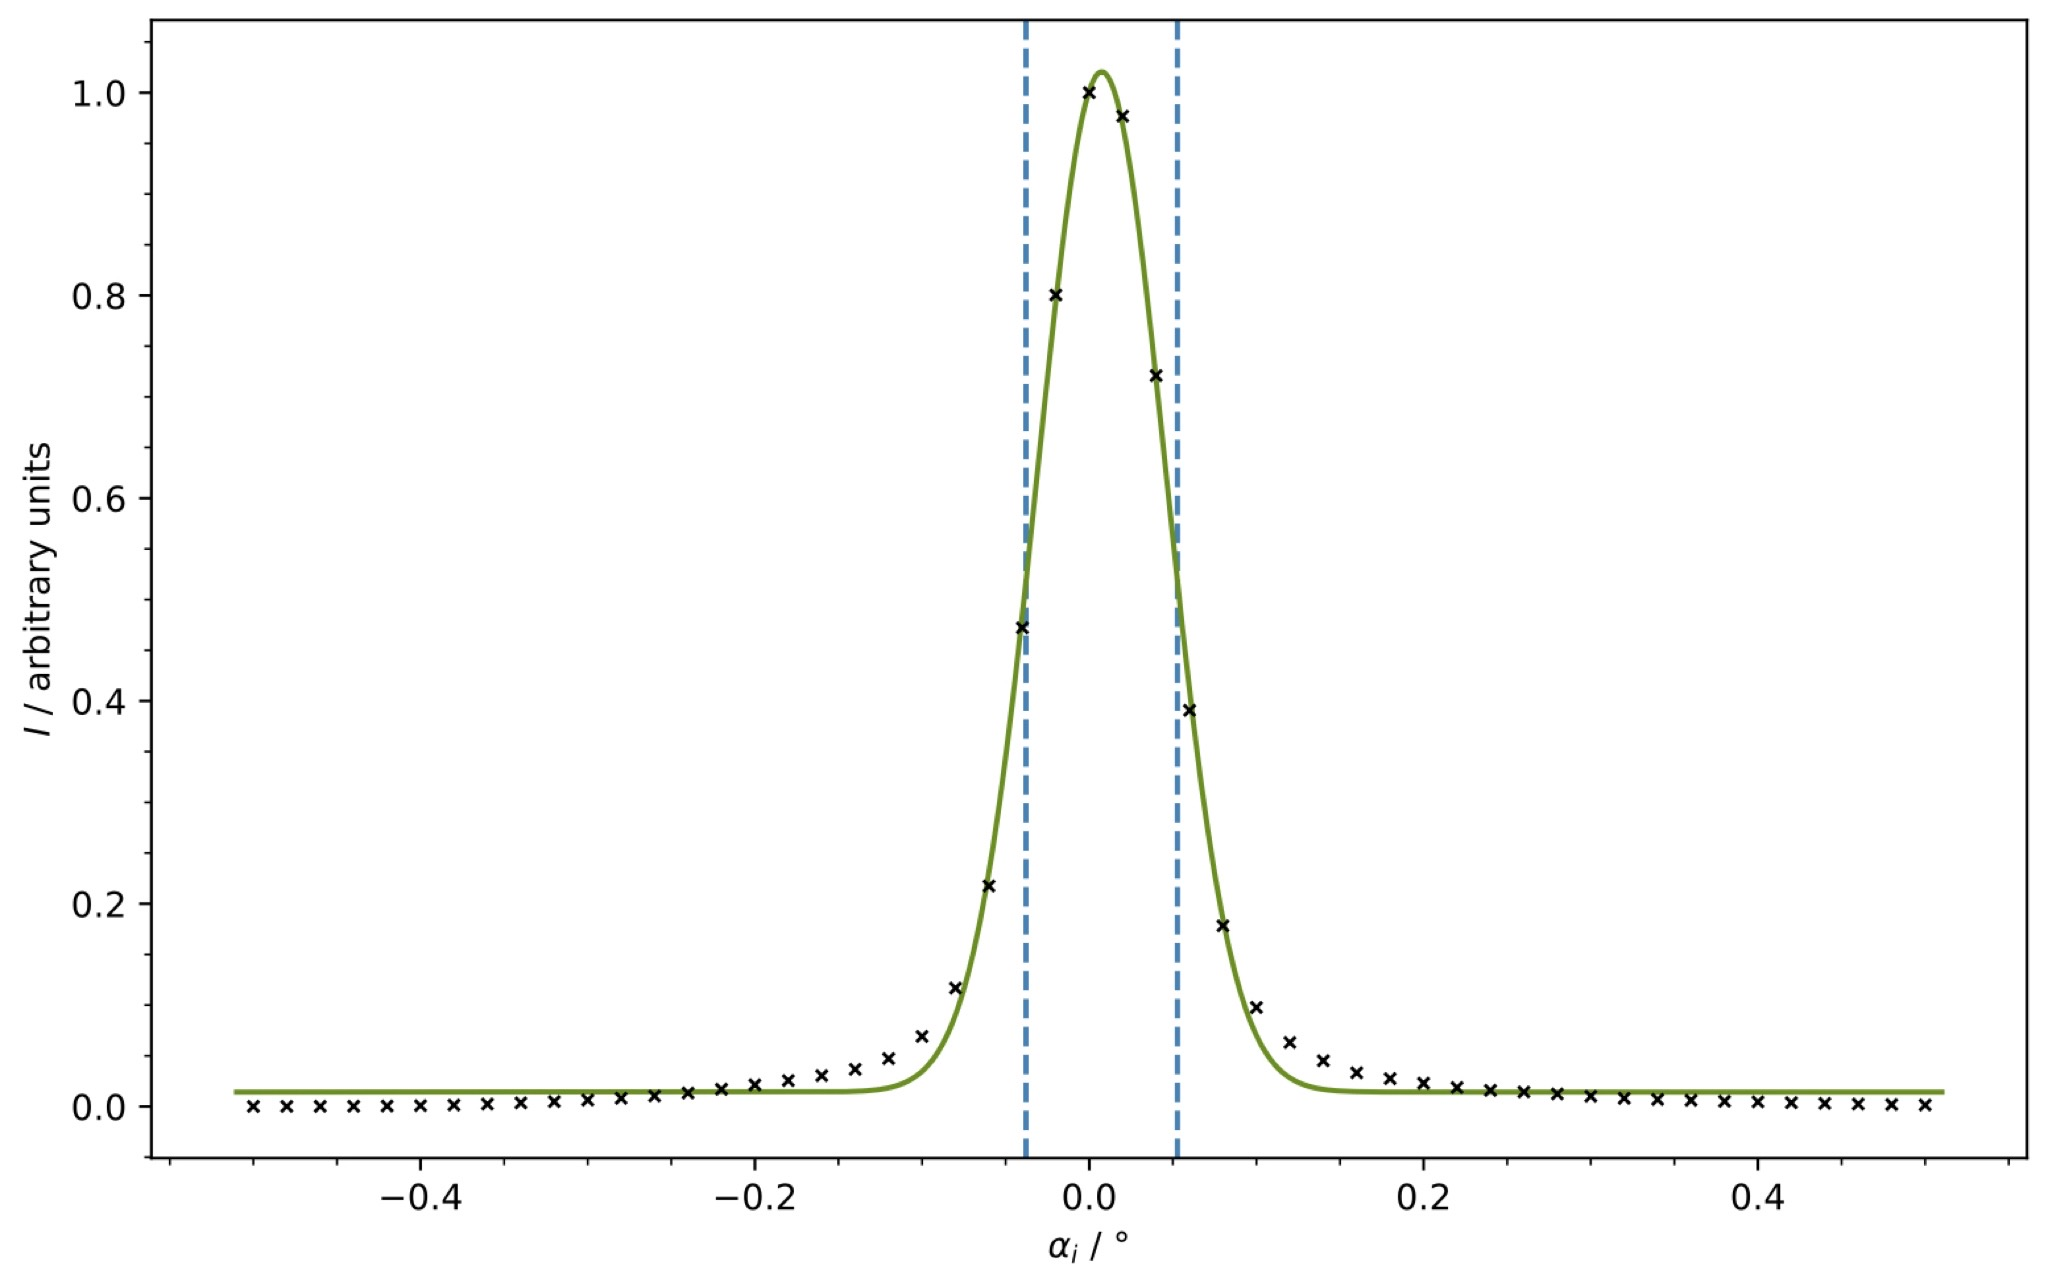
\includegraphics[width=0.88\textwidth]{content/plots/1.jpg}
	\caption{Detector-Scan with fitted Gaussian and marked half maximum positions.}
	\label{fig:detector-scan}
\end{figure}

The curve fit to this function shown in Figure \ref{fig:detector-scan} yields parameters
\begin{align*}
	a &= \num{1.01+-0.01} \: , & b &= \num{0.014+-0.002} \: , \\
	\mu &= \qty{0.0074+-0.0004}{\degree} \: , & \sigma &= \qty{0.0385+-0.0005}{\degree} \: .
\end{align*}
One then finds the maximum at $\alpha_{i, \text{max}} = \mu$ as $G(\alpha_{i, \text{max}}) = \num{1.02+-0.01}$
and full width half maximum at $\alpha_{i, \text{fwhm}}^\pm = \mu \pm \sigma \sqrt{2 \ln 2}$ with
\begin{align*}
	\alpha_{i, \text{fwhm}}^+ = \qty{-0.0528+-0.0007}{\degree} \: , &&
	\alpha_{i, \text{fwhm}}^- = \qty{-0.0379+-0.0007}{\degree} \: .
\end{align*}
Following the detector calibration, the sample position is adjusted. When adjusting the vertical coordinate, one identifies the difference
between maximum to minimum intensity, representing zero to full beam obstruction, with the beam width. As indicated in Figure~\ref{fig:z-scan},
a value
\begin{equation*}
	\tilde{d} = \qty{0.24+-0.06}{\milli\meter}
\end{equation*}
is determined.

\begin{figure}[H]
	\centering
	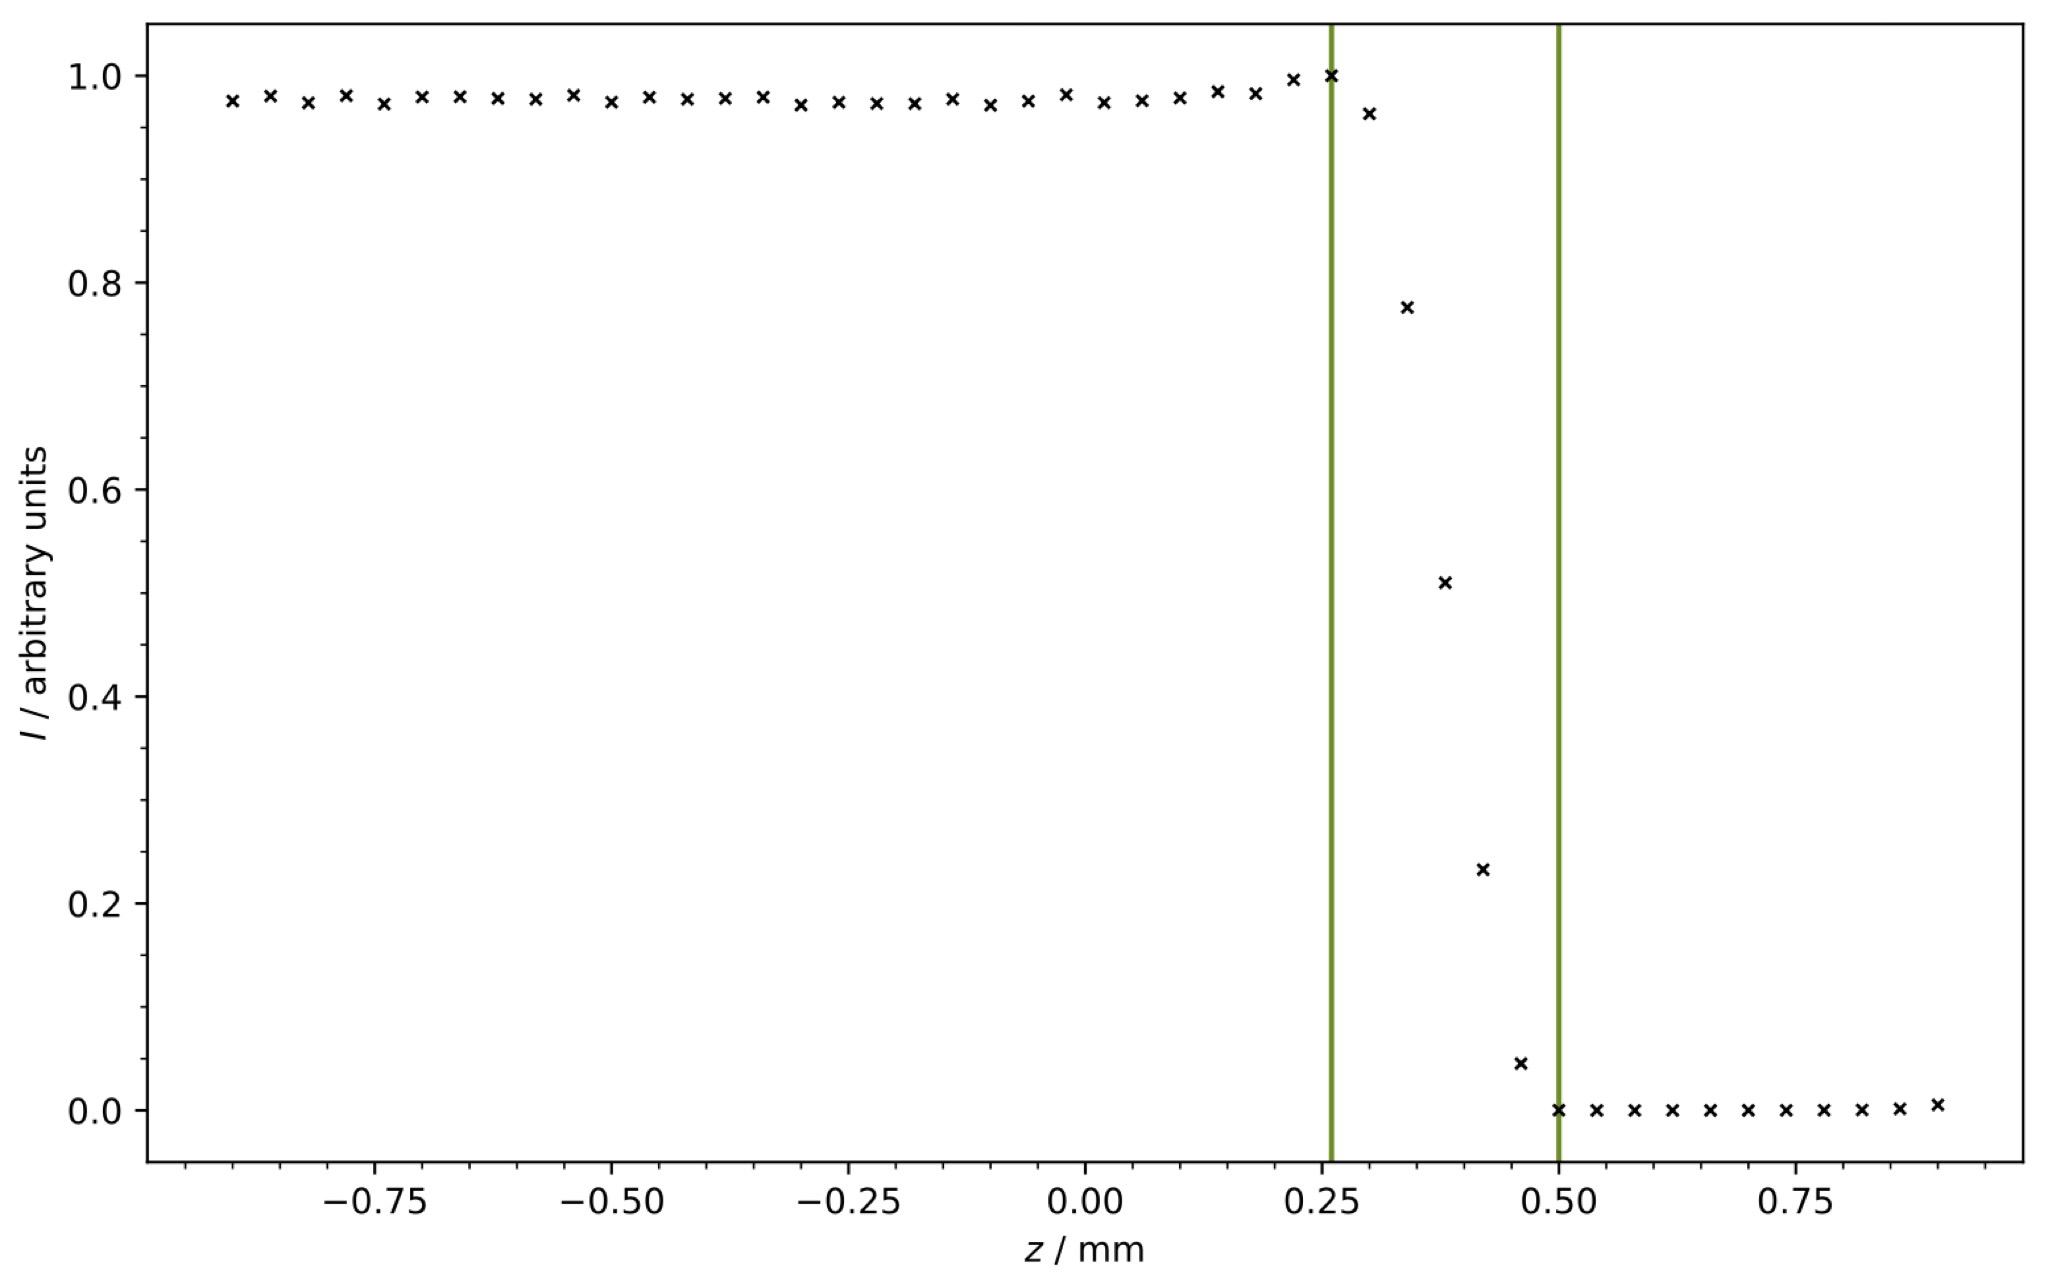
\includegraphics[width=0.88\textwidth]{content/plots/2.jpg}
	\caption{Z-Scan with indicated beam width.}
	\label{fig:z-scan}
\end{figure}

From the intensity valley during horizontal shifting, Figure \ref{fig:x-scan} leads to a sample size
\begin{equation*}
	D = \qty{21+-3}{\milli\meter} \: ,
\end{equation*}
which is in agreement with the literature value $D = \qty{20}{\milli\meter}$ \cite{xray}. From equation \eqref{eqn:geom-angle} follows a
geometry angle
\begin{equation*}
	\alpha_{g, 1} = \qty{0.7+-0.2}{\degree} \: .
\end{equation*}

\begin{figure}[H]
	\centering
	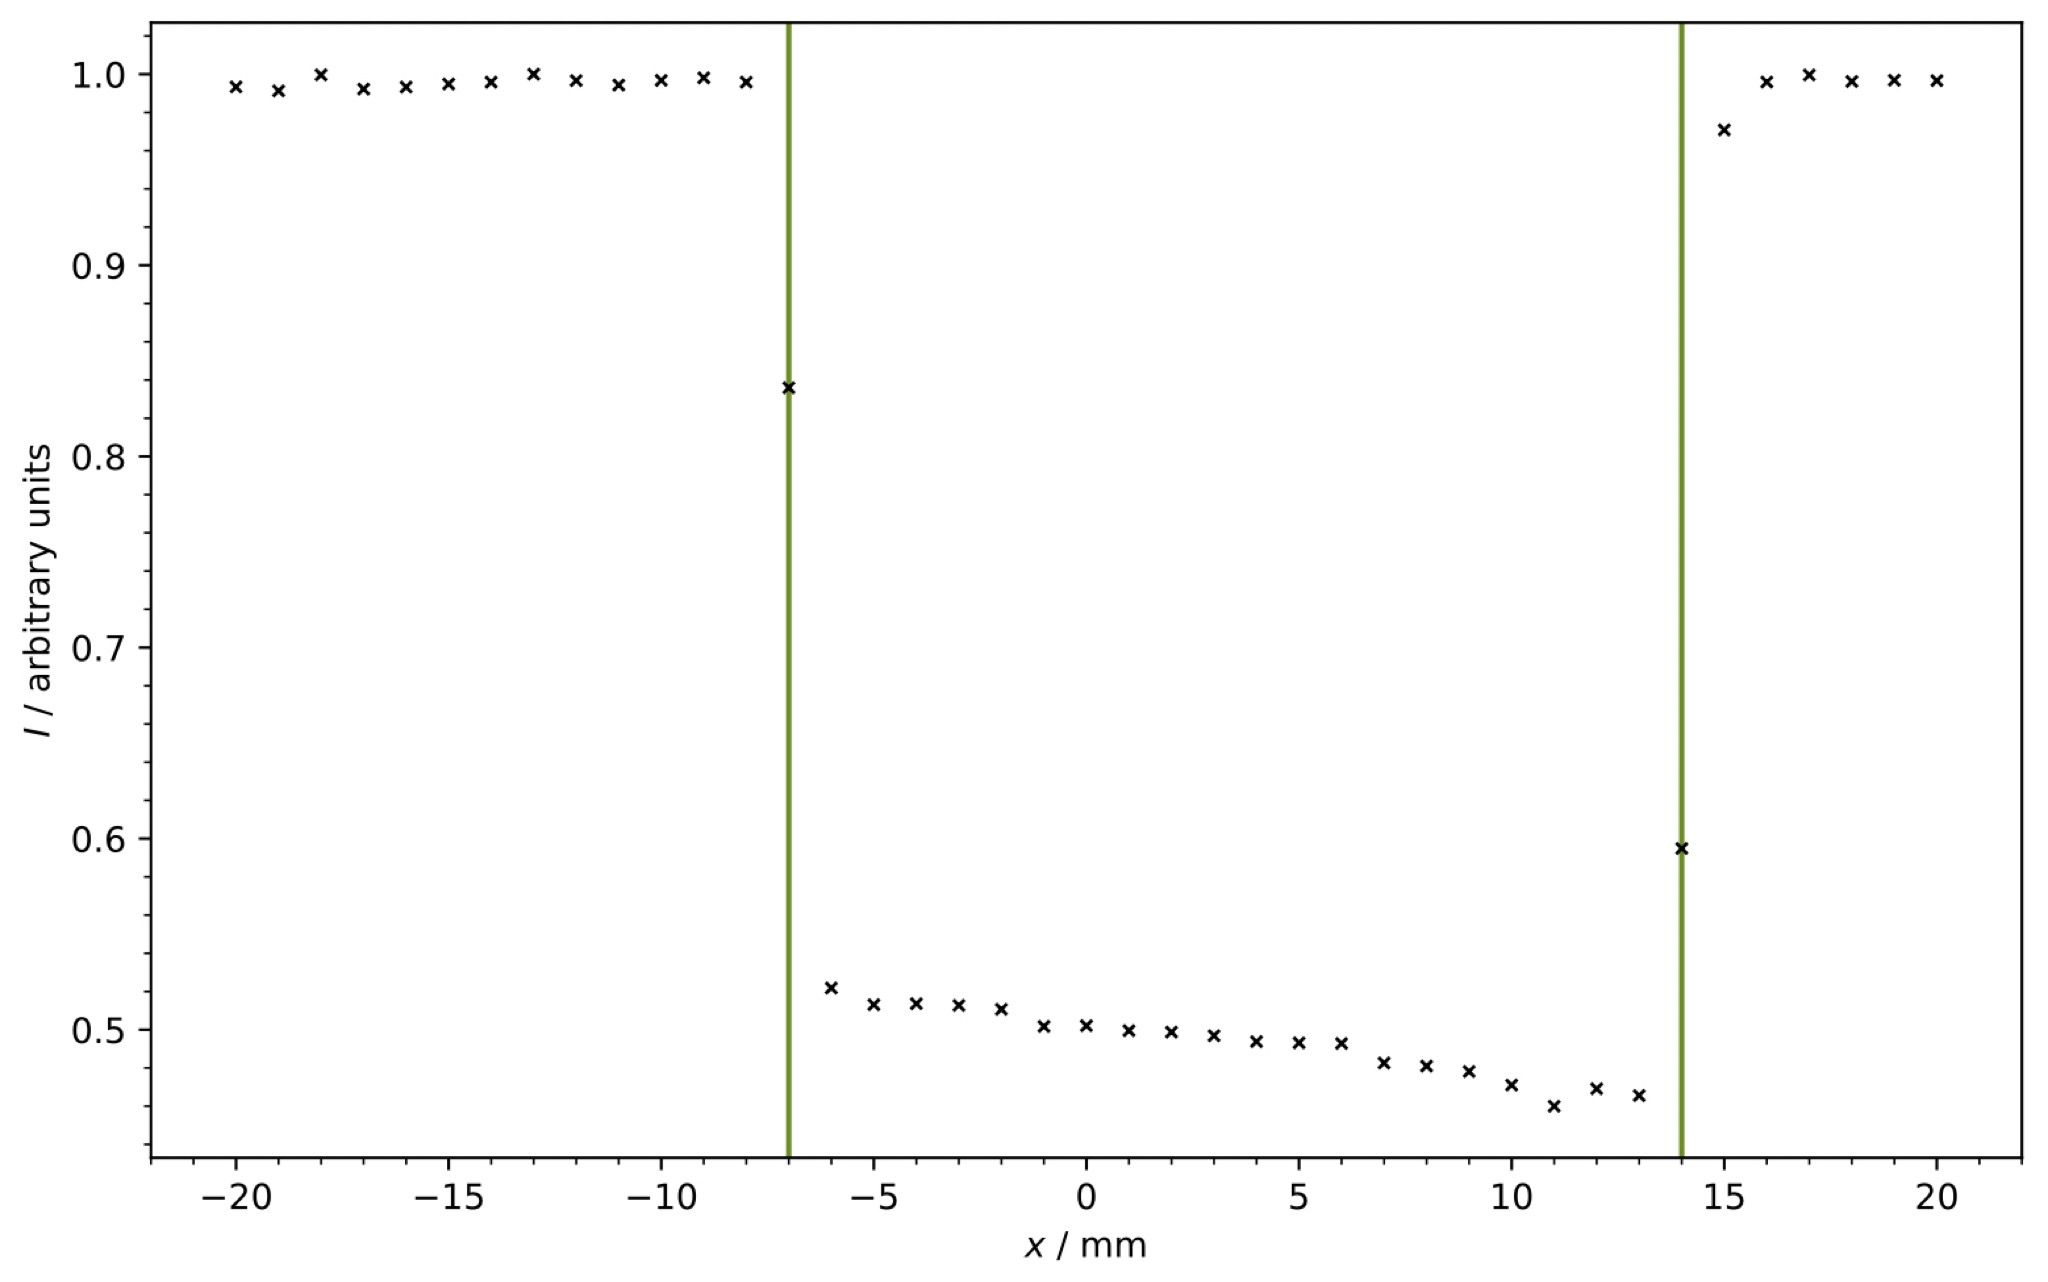
\includegraphics[width=0.88\textwidth]{content/plots/3.jpg}
	\caption{X-Scan with indicated sample size.}
	\label{fig:x-scan}
\end{figure}

Reading the geometry angle from Figure \ref{fig:rocking-curve}, a somewhat lower value of
\begin{equation*}
	\alpha_{g, 2} = \qty{0.54+-0.03}{\degree}
\end{equation*}
is obtained, though it still falls inside the uncertainty of the previous result.


\begin{figure}[H]
	\centering
	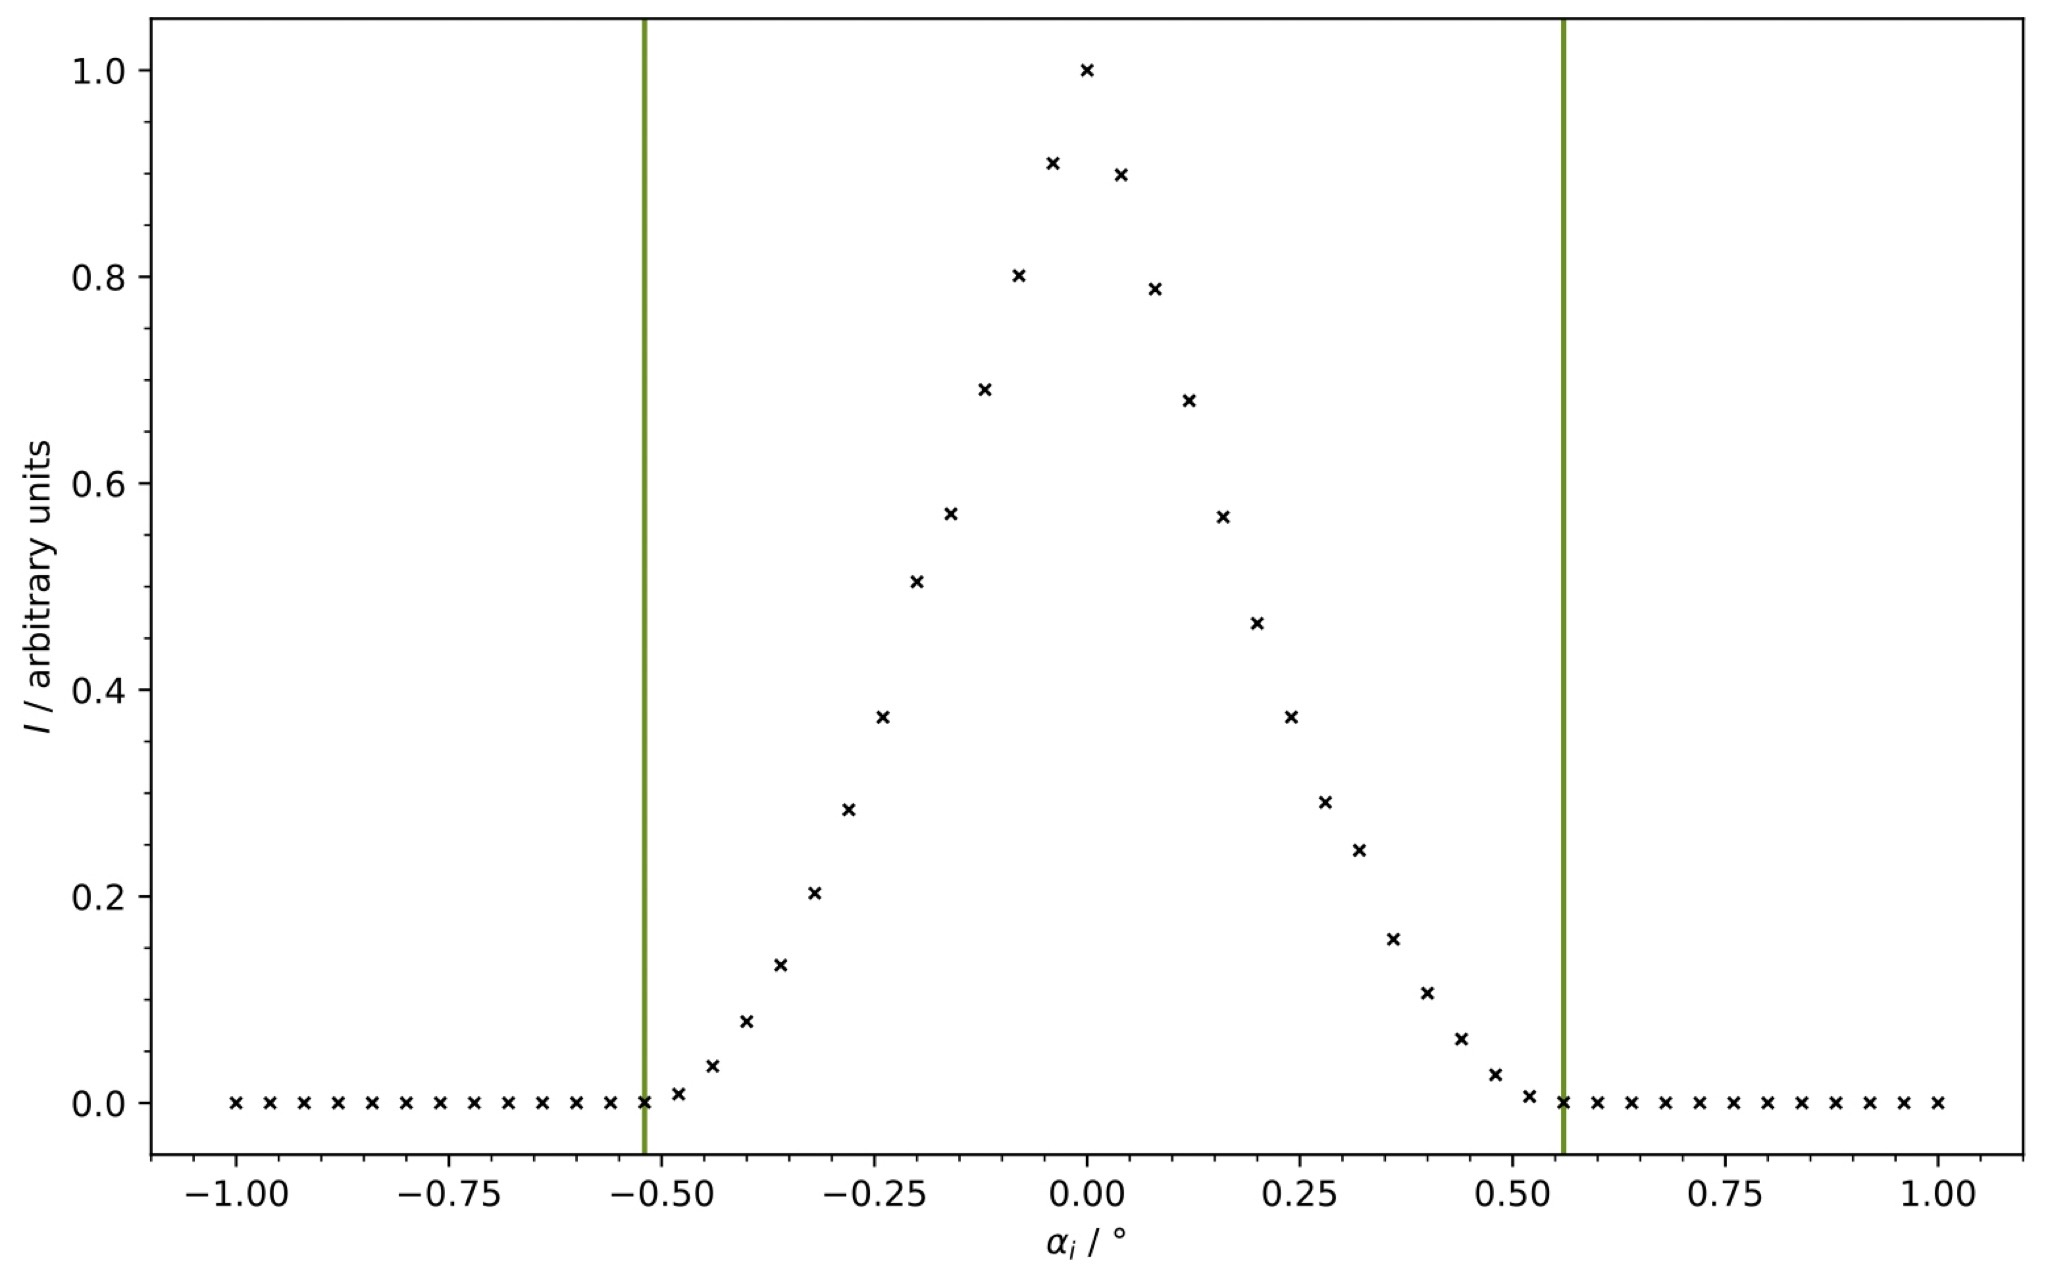
\includegraphics[width=0.88\textwidth]{content/plots/4.jpg}
	\caption{Rocking-Curve with geometry angles.}
	\label{fig:rocking-curve}
\end{figure}



\subsection{Measurement}

\begin{figure}[H]
	\centering
	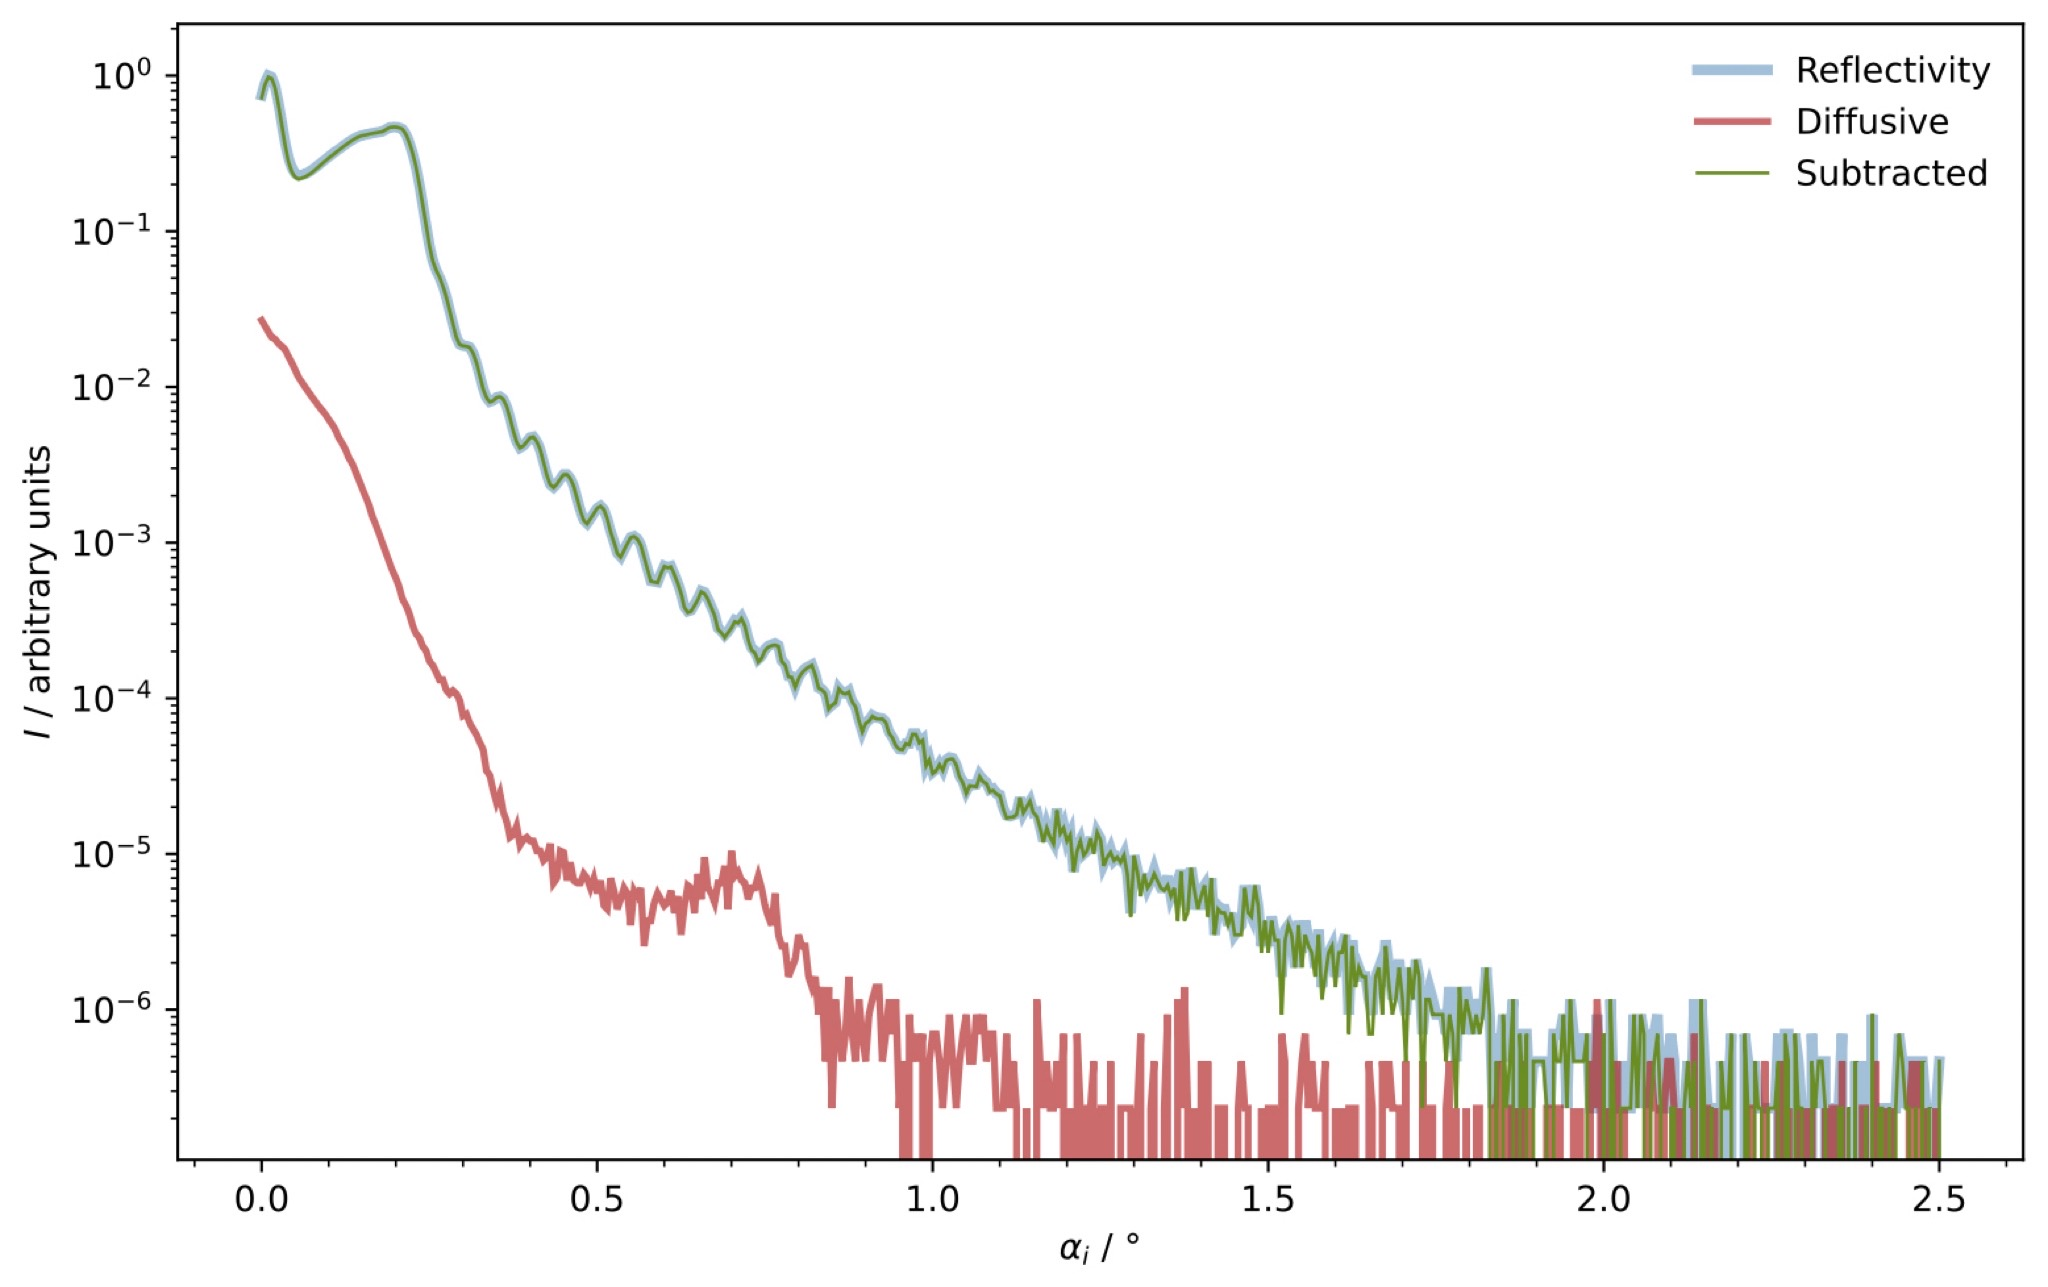
\includegraphics[width=0.88\textwidth]{content/plots/5.jpg}
	\caption{Intensity curves for reflectivity and diffusive background.}
	\label{fig:reflex-diffuse}
\end{figure}

\begin{figure}[H]
	\centering
	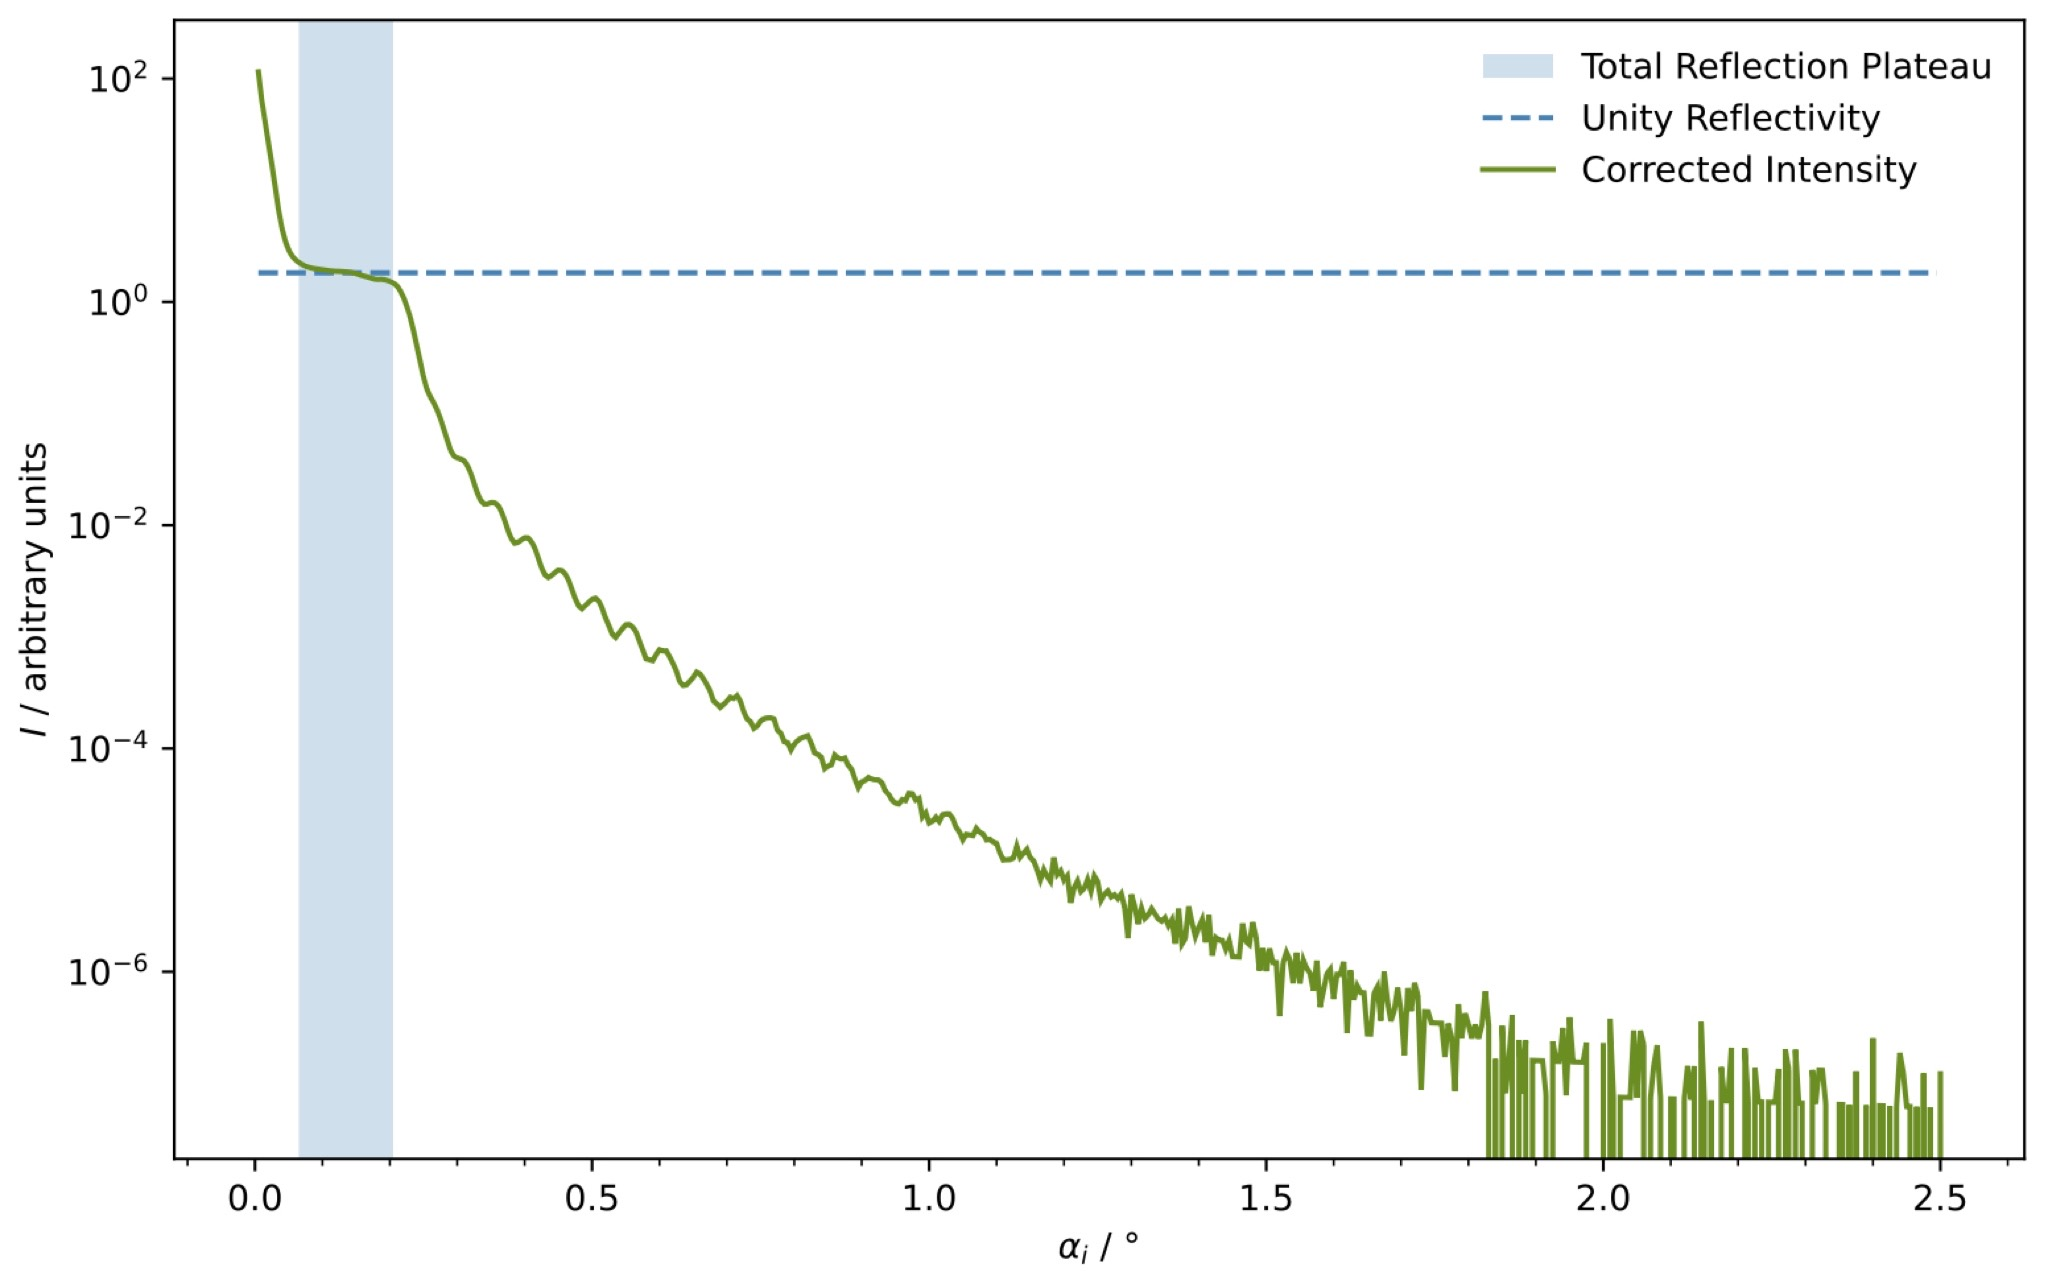
\includegraphics[width=0.88\textwidth]{content/plots/6.jpg}
	\caption{Intensity after geometry factor correction and region of total reflection.}
	\label{fig:geom-corr}
\end{figure}

\begin{figure}[H]
	\centering
	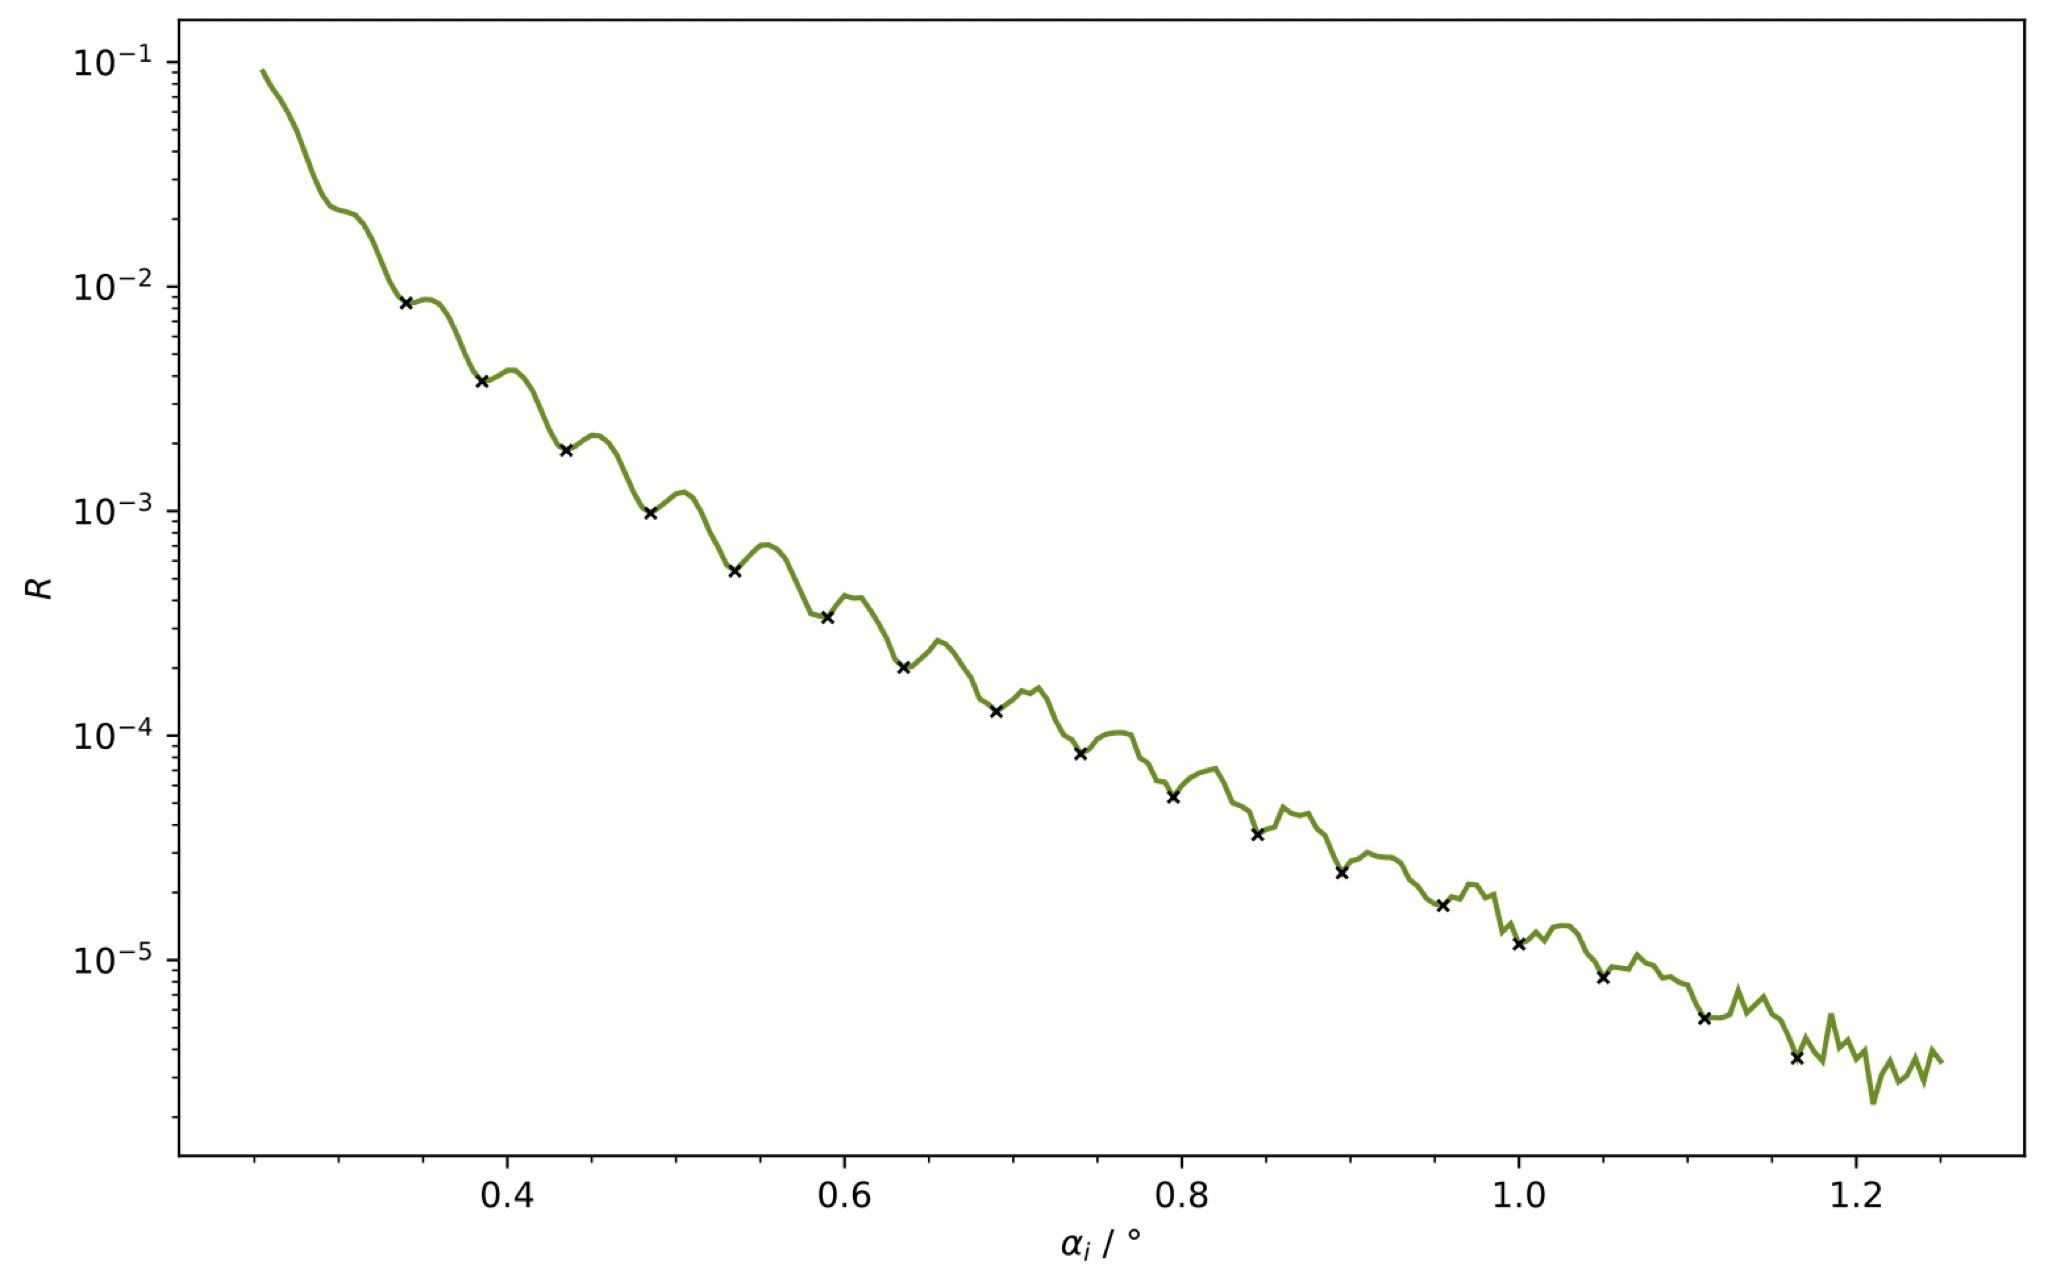
\includegraphics[width=0.88\textwidth]{content/plots/7.jpg}
	\caption{Detailed reflectivity curve with Kiessig oscillation minima.}
	\label{fig:kiessig-peaks}
\end{figure}

\begin{figure}[H]
	\centering
	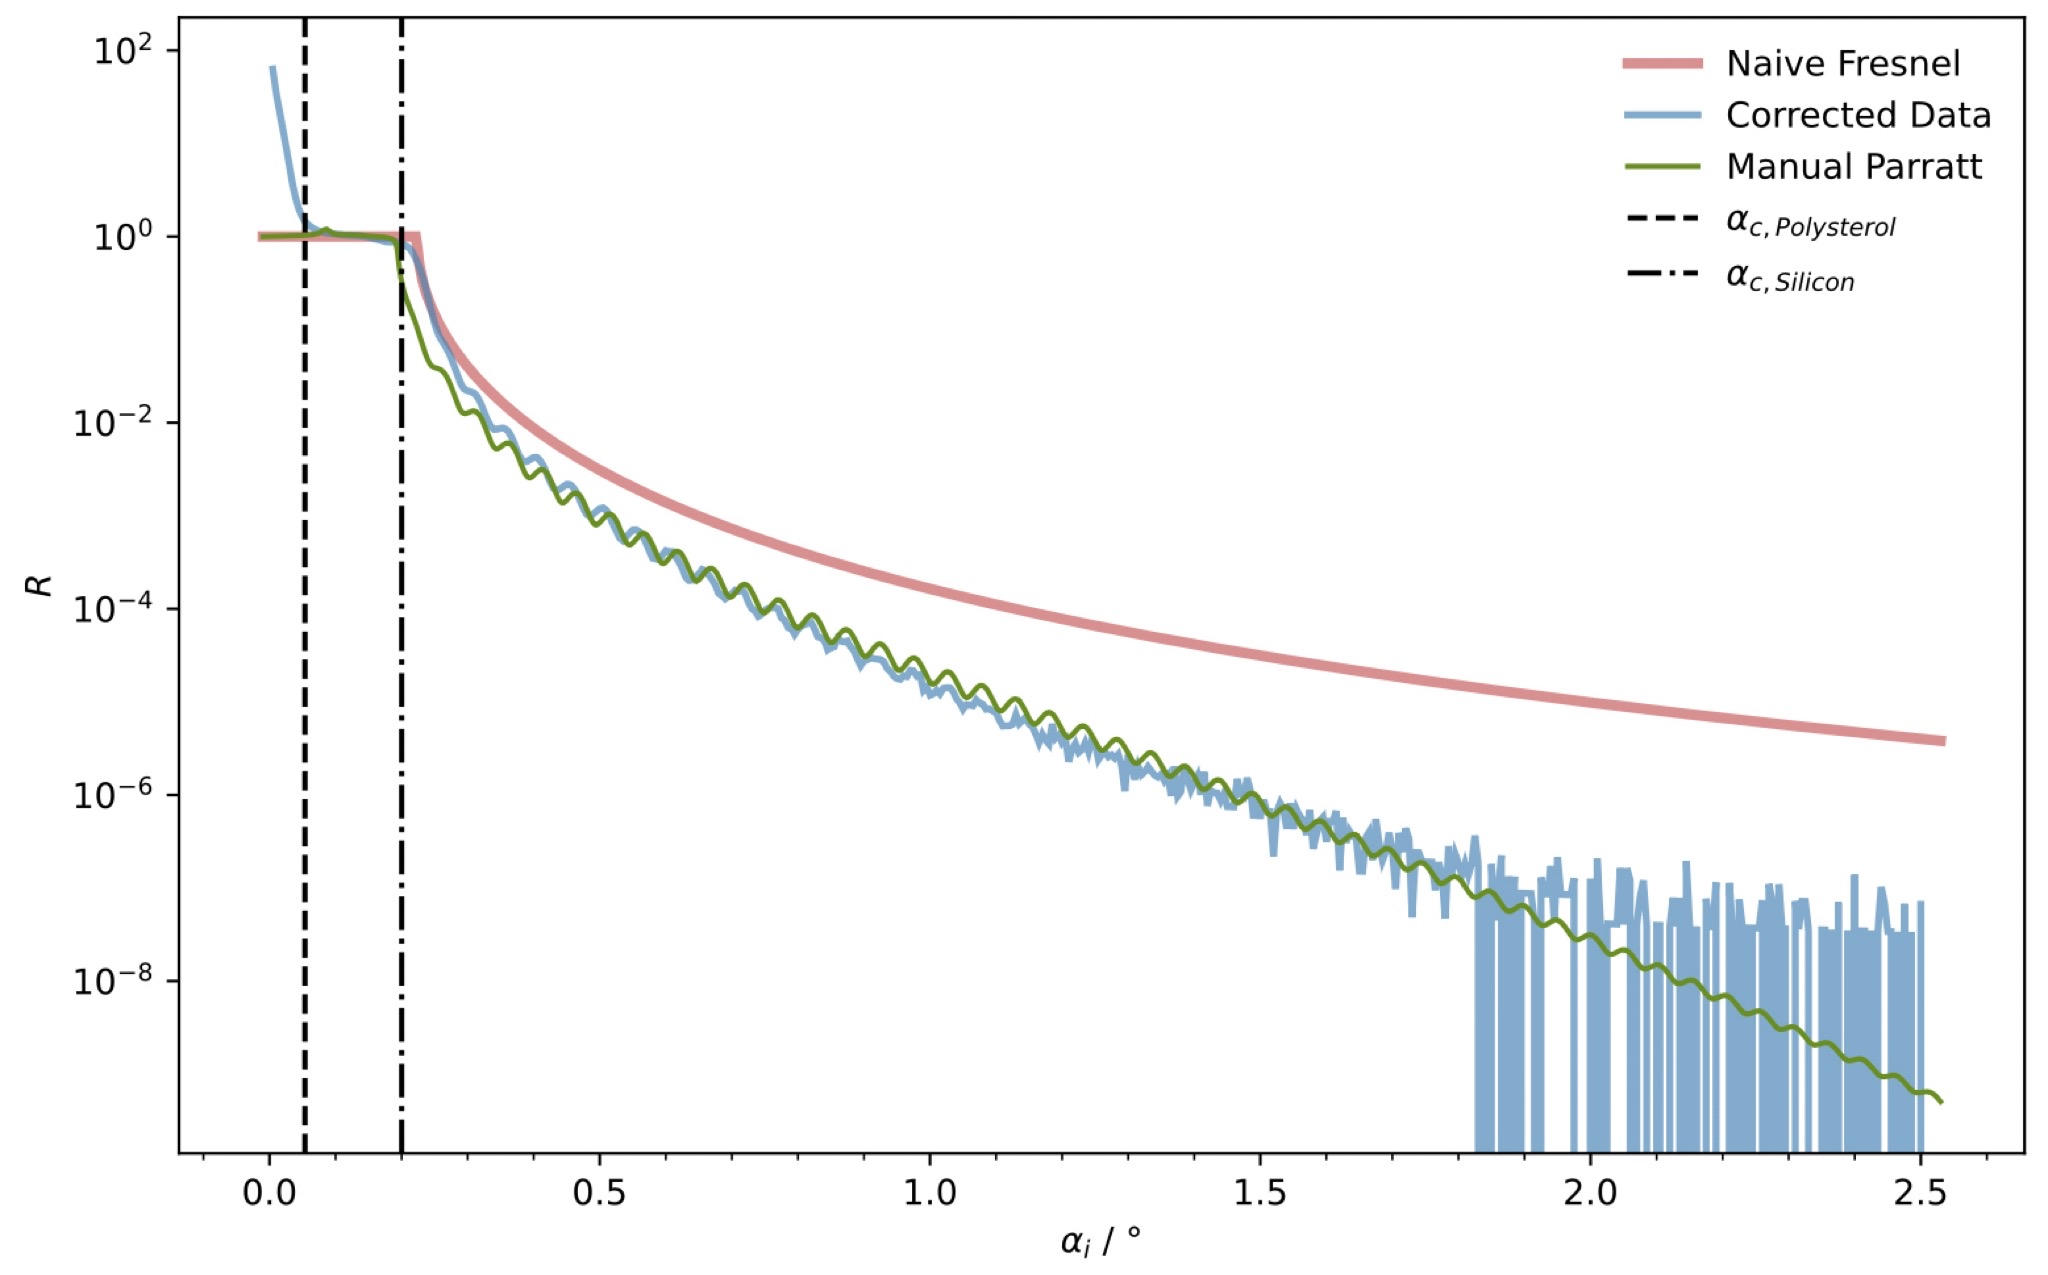
\includegraphics[width=0.88\textwidth]{content/plots/8.jpg}
	\caption{Full reflectivity curve with Parratt and Fresnel fits.}
	\label{fig:parratt-fresnel}
\end{figure}
